
% Hier steht der Rezepttitel
\section{Dulce di Leche Creme}
% Untertitel
% Danach die Zutaten in Tabellenform
% Wie viele werden satt?
\begin{minipage}{0.45\textwidth}
  \flushleft
  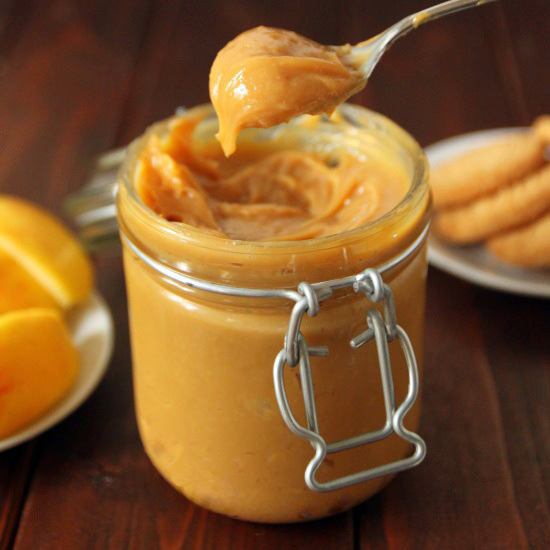
\includegraphics[width=0.7\textwidth]{dulce.jpg}
\end{minipage}
\begin{minipage}{0.55\textwidth}
Yields about 1$\nicefrac{3}{4}$-2 cups of sweet cream.
%\textbf{Zutaten:}
\begin{table}[H]
\centering
% eine Tabelle mit insgesamt 4 Spalten, falls mehr Zutaten benoetigt werden
% links: Menge, rechts: Zutat
\begin{tabular*}{1\textwidth}{rlrl}
%& && \\
3 cups  & whole milk & 1 cup & sugar \\
1$\nicefrac{1}{2}$ cups & cream & 2 pinches & salt \\
\end{tabular*}
\end{table}
\end{minipage}
%Zubereitung:
\begin{Notes}
\item Mix all ingredients in a pot and bring to a boil uncovered. Stirring constantly, let boil lighlty until thickend to desired consistency (creamy) and the color turns golden. Watch out, it's going to get even more firm when it cools down!
\item Tip: Reducing to about $\nicefrac{1}{3}$ of the initial volume is a good rule of thumb. In these quantities this will take about one hour, during which the pot cannot stay unobserved.
\item Store in the fridge.
\end{Notes}
\newpage
% Hier steht der Rezepttitel
\section*{Dulce di Leche-Creme}
% Untertitel
% Danach die Zutaten in Tabellenform
% Wie viele werden satt?
\begin{minipage}{0.55\textwidth}
Für etwa 400\,ml süße Creme
%\textbf{Zutaten:}
\begin{table}[H]
\centering
% eine Tabelle mit insgesamt 4 Spalten, falls mehr Zutaten benoetigt werden
% links: Menge, rechts: Zutat
\begin{tabular*}{1\textwidth}{rlrl}
%& && \\
800\,ml & Vollmilch & 200\,g & Zucker \\
400\,ml & Sahne & 2 Prisen & Salz \\
\end{tabular*}
\end{table}
\end{minipage}
\begin{minipage}{0.45\textwidth}
  \flushright
  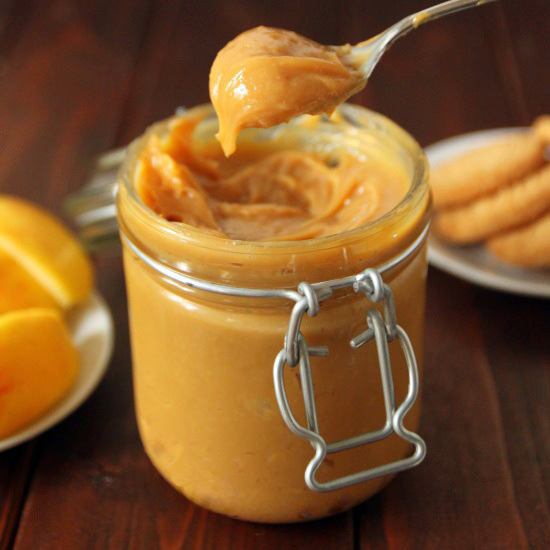
\includegraphics[width=0.7\textwidth]{dulce.jpg}
\end{minipage}
%Zubereitung:
\begin{Notes}
\item Alle Zutaten ohne Deckel in einem Topf zum Kochen bringen. Unter Rühren köcheln lassen, bis es auf die gewünschte Konsistenz (cremig) und Farbe (goldgelb) eingekocht ist. Achtung, es wird noch fester, wenn es abkühlt! 
\item Tipp: Auf etwa $\nicefrac{1}{3}$ der Ausgangsmenge zu reduzieren ist eine gute Daumenregel. Das dauert bei dieser Menge etwa eine Stunde, bei der man den Topf nicht unbeaufsichtigt lassen kann. 
\item Im Kühlschrank aufbewahren.
\end{Notes}
\newpage






